% WaRS paper draft — IEEE conference format (IEEEtran). Compile: pdflatex main && bibtex main && pdflatex main ×2
% Scope (06/11/2026, Hậu): MODS-only evaluation; USV-VN, YOLOv8n and power measurement removed
% (previous draft: archive/main_2026-11-06_usvvn_yolo.tex). LaRS only as a short domain-gap study.
% RULE: every number in this paper must trace to a run with run_info.json (commit, config, GPU) or to a
%       result file in results/ / docs/data/. Placeholders are marked \tbd{...} and print in red.
% Naming (Q-010/Q-011): eWaSR-Lite = D-mixer + reduced MLPs (E7, code ewasr_h_lite);
%       eWaSR-Lite (S-mixer) = E6 (ewasr_lite); eWaSR (D-mixer) = E2 (ewasr_h); eWaSR = E1 (ewasr).
\documentclass[conference]{IEEEtran}
\IEEEoverridecommandlockouts
\usepackage{cite}
\usepackage{amsmath,amssymb,amsfonts}
\usepackage{graphicx}
\usepackage{booktabs}
\usepackage{multirow}
\usepackage{xcolor}
\usepackage{url}
\newcommand{\tbd}[1]{\textcolor{red}{[#1]}}
\newcommand{\figplaceholder}[2]{\fbox{\parbox[c][#2][c]{0.95\linewidth}{\centering\small\textcolor{red}{#1}}}}
\newcommand{\pmstd}[2]{#1{\scriptsize$\pm$#2}}

\begin{document}

\title{eWaSR-Lite: Real-Time Maritime Obstacle Segmentation for Low-Cost USVs on Raspberry Pi~5 and Hailo-8L}

\author{\IEEEauthorblockN{\tbd{Author 1}}
\IEEEauthorblockA{\tbd{Affiliation}\\
\tbd{email}}
\and
\IEEEauthorblockN{\tbd{Advisor}}
\IEEEauthorblockA{\tbd{Affiliation}\\
\tbd{email}}}

\maketitle

\begin{abstract}
Small unmanned surface vehicles (USVs) need to detect the obstacles they must avoid in real time on inexpensive hardware, including obstacle types never seen during training. Segmentation networks such as eWaSR meet the second requirement by labelling every pixel as water, sky or obstacle, but have not been studied on low-cost dataflow accelerators. We deploy eWaSR on the Hailo-8L (13~TOPS) of a Raspberry~Pi~5 and find that its speed is limited not by unsupported operators but by the number of compiler contexts, which is driven by the channel MLPs of the feature mixer. The published eWaSR weights have silenced five of these six MLPs (layer scale $\approx\!10^{-40}$), so the compiler drops them; when the network is retrained from ImageNet they remain active and double the number of contexts. Removing them structurally (eWaSR-Lite) cuts the parameters by 61\% and the contexts from 8 to 4, and makes the network 59--70\% faster on the accelerator (29.7 vs 17.5--18.8~FPS) and 43--55\% faster end-to-end (22.7 vs 14.6--15.8~FPS on MODS frames) with unchanged accuracy on MODS (F1 92.1$\pm$0.3 vs 91.8$\pm$0.7\% over three training runs). eWaSR-Lite is also robust to INT8 post-training quantization: across three calibration sets its danger-zone F1 on the device stays within 85.1--85.7\%, whereas that of eWaSR drops to 37--86\%, a failure that pixel agreement with the FP32 model does not reveal. Finally, we show that retraining on LaRS reduces false alarms on river water from 19\% to 1.6\% of water pixels. Code and evaluation tools are released at \tbd{URL}.
\end{abstract}

\begin{IEEEkeywords}
unmanned surface vehicle, obstacle detection, semantic segmentation, edge AI, INT8 quantization, Hailo-8L
\end{IEEEkeywords}

%==============================================================================
\section{Introduction}
%==============================================================================
Unmanned surface vehicles (USVs) are increasingly used for water-quality monitoring, surveys and waste collection on rivers, lakes and coastal waters. To navigate autonomously, a USV must detect the obstacles it has to avoid, from boats to small buoys, on hardware that fits the cost and power budget of a small vessel. This paper addresses the perception part of obstacle avoidance: the output is a list of obstacles on the water surface with their bearings, to be consumed by a separate planner.

Object detectors such as YOLO~\cite{redmon2016yolo,jocher2023yolov8} are fast and well supported by edge toolchains, but report only the classes they were trained on. Maritime obstacle segmentation networks such as WaSR~\cite{bovcon2022wasr} and its embedded successor eWaSR~\cite{tersek2023ewasr} instead label every pixel as \emph{water}, \emph{sky} or \emph{obstacle}, so anything that is neither water nor sky is reported. Trained on MaSTr1325~\cite{bovcon2019mastr} and evaluated on MODS~\cite{bovcon2022mods}, eWaSR runs on an OAK-D device~\cite{tersek2023ewasr}.

Two questions remain open for low-cost USVs. First, eWaSR was designed for the Myriad~X VPU. It has not been evaluated on dataflow accelerators such as the Hailo-8L, now available as an add-on for the Raspberry~Pi~5, which impose their own constraints on operators, static shapes and on-chip memory. Second, deployment on such accelerators requires INT8 post-training quantization, and whether the resulting accuracy is stable, in particular for obstacles close to the vessel, has not been reported.

This paper makes the following contributions:
\begin{itemize}
\item \textbf{eWaSR-Lite}, a variant of eWaSR for the Hailo-8L. We show that the feature-mixer MLPs, not unsupported operators, set the number of compiler contexts, and that whether these MLPs vanish during training depends on the training recipe: the published weights silence five of six, our ImageNet-initialised runs do not. Removing the five MLPs makes speed independent of this: in a controlled $2\times2$ study (spatial mixer S or depthwise gate D, full or reduced MLPs, one quantization protocol) it cuts the parameters by 61\%, the contexts from 8 to 4, and raises the accelerator throughput by 49--86\% with no loss of MODS accuracy beyond the run-to-run spread (Sec.~\ref{sec:method},~\ref{sec:fp32},~\ref{sec:hw}).
\item An \textbf{INT8 robustness study} on the Hailo Dataflow Compiler, evaluated on the device with the official MODS toolkit. The INT8 accuracy of eWaSR depends strongly on the calibration set, through false obstacles in front of the vessel, while eWaSR-Lite is stable; pixel agreement between INT8 and FP32 masks, a common sanity check, misses these failures (Sec.~\ref{sec:quant}).
\item An open-source pipeline from training to on-device inference on Raspberry~Pi~5, and a short study of the domain gap between the maritime training data and river scenes on LaRS~\cite{zust2023lars} (Sec.~\ref{sec:lars}).
\end{itemize}

%==============================================================================
\section{Related Work}
%==============================================================================
\textbf{Maritime obstacle segmentation.} WaSR~\cite{bovcon2022wasr} builds on a DeepLab-style ResNet-101 encoder~\cite{chen2018deeplab,he2016resnet} and a decoder that fuses encoder features with attention refinement modules; it is trained with a focal loss~\cite{lin2017focal} and a water-obstacle separation loss. eWaSR~\cite{tersek2023ewasr} replaces the encoder with ResNet-18 and the decoder with a TopFormer-style~\cite{zhang2022topformer} design in which MetaFormer blocks~\cite{yu2022metaformer} operate on a small pyramid of pooled tokens and semantic injection modules re-inject global context into each scale. MaSTr1325~\cite{bovcon2019mastr} is the standard training set; MODS~\cite{bovcon2022mods} provides an obstacle- and water-edge-based evaluation protocol with a danger zone; LaRS~\cite{zust2023lars} extends training and evaluation to more diverse scenes, including rivers and lakes.

\textbf{Efficient segmentation.} Real-time segmentation networks reduce cost by splitting spatial detail and context into separate paths~\cite{yu2018bisenet} or by computing global context on a coarse token grid~\cite{zhang2022topformer}. Most are designed for mobile GPUs or CPUs; we target a fixed-function INT8 dataflow accelerator, where operator support and on-chip memory matter more than FLOPs.

\textbf{Quantization for edge accelerators.} Integer-only inference~\cite{jacob2018quantization} and the post-training and quantization-aware recipes summarised in~\cite{krishnamoorthi2018quantizing,nagel2021white} underlie vendor toolchains such as the Hailo Dataflow Compiler~\cite{hailo_dfc}. Prior maritime work reports quantized results on the OAK-D~\cite{tersek2023ewasr} for a single calibration; we are not aware of a study of calibration-set sensitivity for maritime segmentation. \tbd{verify against recent literature before submission}

%==============================================================================
\section{Method}
\label{sec:method}
%==============================================================================
\subsection{Constraints of the Hailo-8L}
The Hailo-8L executes a compiled, statically shaped dataflow graph in INT8. Layers that the compiler cannot map must run on the host, which splits the network and adds PCIe transfers. When the weights do not fit in on-chip memory, the network is partitioned into several \emph{contexts} that are swapped at run time, which reduces throughput. With the Hailo Dataflow Compiler (DFC) 3.34, the original eWaSR, including the channel-wise \texttt{ReduceMean}/\texttt{ReduceMax} of its spatial attention, parses and runs entirely on the accelerator. Its speed is limited by the number of contexts instead (Table~\ref{tab:hw}), and that number depends on how many of the feature-mixer MLPs are active.

\subsection{From eWaSR to eWaSR-Lite}
\label{sec:lite}
Fig.~\ref{fig:arch} shows the architecture. We keep the ResNet-18 encoder of eWaSR without the IMU input, the pyramid pooling of four encoder stages (strides 4--32) to a $\lceil H/64\rceil\times\lceil W/64\rceil$ token grid ($6\times8$ for a $384\times512$ input, 960 channels), the feature mixer of six MetaFormer blocks on these tokens, the long-skip enricher of two MetaFormer blocks on the stride-8 features, and the four semantic injection modules. Each MetaFormer block computes
\begin{align}
x &\leftarrow x + \gamma_1 \odot \mathrm{Mixer}(\mathrm{BN}(x)),\\
x &\leftarrow x + \gamma_2 \odot \mathrm{MLP}(\mathrm{BN}(x)),
\end{align}
with batch normalization instead of layer normalization and learnable per-channel layer scales $\gamma_1,\gamma_2$ initialised to $10^{-5}$. eWaSR uses two kinds of token mixer, both of the form $y = A(x)\odot x$. The channel mixer (C) is an attention refinement module~\cite{yu2018bisenet}, $A_C(x)=\sigma(\mathrm{BN}(W\,\mathrm{GAP}(x)))\in\mathbb{R}^{C\times1\times1}$. The spatial mixer (S) computes
\begin{equation}
A_S(x)=\sigma\!\left(k_{3\times3} * \left[\operatorname{mean}_c x;\ \operatorname{max}_c x\right]\right)\in\mathbb{R}^{1\times H\times W}.
\end{equation}
eWaSR uses the mixer sequence CCCCSS and an SS enricher.

\textbf{Silenced MLPs.} Each feature-mixer MLP maps 960 to 3840 channels and back (7.4\,M parameters), so the six MLPs hold 44.3\,M of the 60.3\,M parameters of eWaSR. In the published eWaSR weights~\cite{tersek2023ewasr}, the mean $|\gamma_2|$ of blocks 1--5 is about $3.6\times10^{-40}$, a denormal value; only the MLP of block~0 contributes to the output (Table~\ref{tab:gamma}). After quantization these branches are exactly zero and the compiled network no longer depends on them: the published weights compile to 5 contexts, and their INT8 masks on all 8175 MODS frames are bit-identical to those of the same weights loaded into the reduced network below. When we train eWaSR from an ImageNet-initialised encoder (Sec.~\ref{sec:training}), the layer scales do not vanish. In each of three runs, one block shrinks to $10^{-8}$--$10^{-13}$ (block~3 in two runs, block~4 in the third) and the others stay between $2.5\times10^{-4}$ and $1.2\times10^{-2}$ (Table~\ref{tab:gamma}). None of these values is zero, so all MLPs stay in the compiled graph and the network needs 8 contexts instead of 4 (Table~\ref{tab:c1}). The published weights were trained with a longer schedule and a larger batch (Sec.~\ref{sec:training}); which factor drives the layer scales to zero is open (Sec.~\ref{sec:disc}).

\textbf{Reduced MLPs.} We remove the MLP branch, together with its normalization and layer scale, from feature-mixer blocks 1--5 and keep it in block~0 and in the enricher. This removes 36.9\,M parameters and 1.77 GMAC (Table~\ref{tab:arch}). Loaded with the published eWaSR weights, the reduced network produces logits identical to eWaSR (maximum absolute difference 0), so the change makes explicit what the original training had converged to, and makes the compact graph independent of the training recipe.

\textbf{Depthwise spatial gate (D).} The spatial mixer reduces along the channel axis, an operation that many accelerators support poorly. We replace it with a gate that uses only convolution, batch normalization and sigmoid:
\begin{equation}
A_D(x)=\sigma\!\left(\textstyle\sum_{c} w_c\,\mathrm{BN}(k_c * x_c) + b\right)\in\mathbb{R}^{1\times H\times W},
\end{equation}
where $k_c$ is a per-channel $3\times3$ depthwise kernel and $w_c$ the weights of a $1\times1$ convolution to a single channel. D keeps the role of S, a single spatial gate broadcast over all channels, but replaces the fixed mean/max pooling over channels with a learned linear combination; it contains the mean branch of S as a special case ($w_c=1/C$, identity $k_c$). The mixer sequence becomes CCCCDD with a DD enricher.

\textbf{eWaSR-Lite} combines both changes (CCCCDD mixer with an MLP only in block~0, DD enricher; 23.38\,M parameters, 10.23 GMAC). We report the four combinations as eWaSR, eWaSR (D-mixer), eWaSR-Lite (S-mixer) and eWaSR-Lite. Removing the MLPs is the first-order effect; the choice between S and D is a second-order effect (Sec.~\ref{sec:hw}).

\textbf{Static, accelerator-friendly resampling.} All internal resampling uses integer scale factors and pooling uses fixed-kernel \texttt{AveragePool} instead of adaptive pooling, so the exported ONNX graph has static shapes. Input height and width must be multiples of 32.

\textbf{Upsampling and normalization off the accelerator.} The network outputs three-class logits at $H/4\times W/4$; bilinear upsampling to image resolution and the arg-max run on the host. ImageNet normalization is folded into the accelerator model script, so the host sends raw RGB \texttt{uint8} frames, which removes a float conversion on the CPU and quarters the input transfer size.

\begin{figure*}[t]
\centering
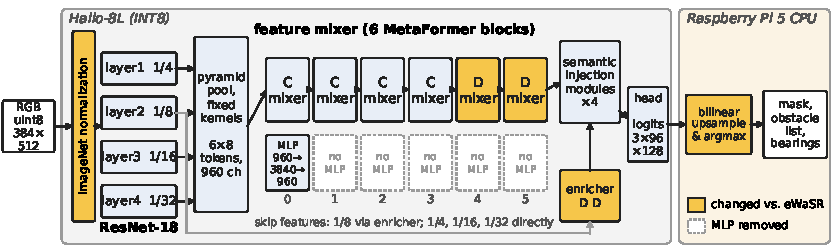
\includegraphics[width=\textwidth]{figs/arch.pdf}
\caption{eWaSR-Lite on Raspberry~Pi~5 + Hailo-8L. Each feature-mixer block is a MetaFormer block (token mixer, then MLP, both with layer scale); the MLPs of blocks 1--5, which hold 61\% of the parameters of eWaSR, are removed, and the spatial mixers S of blocks 4--5 and of the enricher are replaced by the depthwise gate D. ImageNet normalization runs on the accelerator; upsampling of the $H/4$ logits and the arg-max run on the host.}
\label{fig:arch}
% Generated by tools/make_arch_figure.py (third_party/.venv-mods/bin/python); qualitative figure: tools/make_qual_figure.py.
\end{figure*}

\begin{table}[t]
\centering
\caption{Feature-mixer layer scale of the MLP branch, mean $|\gamma_2|$ over channels, per block. Published: eWaSR weights of~\cite{tersek2023ewasr}; E1 s0--s2: eWaSR trained from ImageNet with our recipe, three runs.}
\label{tab:gamma}
\setlength{\tabcolsep}{3pt}
\begin{tabular}{lcccccc}
\toprule
Block & 0 & 1 & 2 & 3 & 4 & 5 \\
\midrule
Published & 1.6e-2 & 3.6e-40 & 3.5e-40 & 3.6e-40 & 3.7e-40 & 3.7e-40 \\
E1 s0     & 1.3e-2 & 8.0e-3 & 5.8e-3 & \textbf{2.0e-9} & 3.2e-3 & 1.2e-2 \\
E1 s1     & 1.1e-2 & 1.0e-2 & 7.5e-4 & 4.5e-3 & \textbf{1.1e-13} & 1.1e-2 \\
E1 s2     & 1.5e-2 & 5.1e-3 & 2.5e-4 & \textbf{2.7e-8} & 7.9e-3 & 9.5e-3 \\
\bottomrule
\end{tabular}
\end{table}
% Source: docs/data/layer_scale_seeds.csv (branch task/T03-recipe, commit 78290c6).

\begin{table}[t]
\centering
\caption{Architecture statistics at $384\times512$ input. GMAC: multiply-accumulates; Reduce: channel-wise \texttt{ReduceMax}/\texttt{ReduceMean} nodes in the exported ONNX graph (feature mixer / enricher).}
\label{tab:arch}
\setlength{\tabcolsep}{3pt}
\begin{tabular}{lcccc}
\toprule
Model & Mixer / enricher & Params & GMAC & Reduce \\
\midrule
eWaSR                    & CCCCSS / SS & 60.25\,M & 11.99 & 4 / 4 \\
eWaSR (D-mixer)          & CCCCDD / DD & 60.28\,M & 11.99 & 0 / 0 \\
eWaSR-Lite (S-mixer)     & CCCCSS / SS & 23.35\,M & 10.22 & 4 / 4 \\
\textbf{eWaSR-Lite}      & CCCCDD / DD & 23.38\,M & 10.23 & 0 / 0 \\
\bottomrule
\end{tabular}
\end{table}
% Source: docs/design.md §6 (08/10/2026); lite rows computed 21/10/2026 with conv/linear MAC hooks.

\subsection{Training}
\label{sec:training}
We follow the eWaSR loss and optimiser~\cite{tersek2023ewasr,bovcon2022wasr}. The loss is $\mathcal{L}=\mathcal{L}_{\mathrm{focal}}+\lambda\mathcal{L}_{\mathrm{sep}}$ with $\lambda=0.01$. The focal loss~\cite{lin2017focal} with $\gamma=2$ is computed after bilinear upsampling of the logits to label resolution; pixels labelled \emph{unknown} in MaSTr1325, and border pixels introduced by geometric augmentation, have an all-zero one-hot target and do not contribute. The separation loss is applied to the stride-16 (layer3) encoder features $f$:
\begin{equation}
\mathcal{L}_{\mathrm{sep}}=\operatorname{mean}_c\frac{N_o\,\sigma^2_{w,c}}{\sum_{i\in O}(f_{i,c}-\mu_{w,c})^2+\varepsilon},
\end{equation}
where $\mu_w,\sigma^2_w$ are the mean and variance of water features in the batch, $O$ the set of obstacle pixels, $N_o=|O|$ and $\varepsilon=0.01$. We use RMSprop (momentum 0.9, $\alpha=0.9$, weight decay $10^{-6}$) with learning rates of $10^{-6}$ for the encoder, $10^{-5}$ for decoder weights and $2\times10^{-5}$ for decoder biases and layer scales, and a polynomial decay with power 0.9 per epoch. Augmentation follows the eWaSR code (horizontal flip, affine shift/scale/rotation, colour jitter, noise). Every model is trained from an ImageNet-pretrained ResNet-18~\cite{he2016resnet} for 100 epochs with batch size 4 and mixed precision on one NVIDIA T4 GPU, and we keep the checkpoint with the highest mIoU on the validation split. The eWaSR paper trains with batch size 16 for up to 200 epochs with early stopping on the validation loss~\cite{tersek2023ewasr}; we use the shorter schedule for all variants so that they can be compared under one recipe within our compute budget.
% T03 (Kaggle V10, submitted 07/11): E1 and E7 with the original recipe (fp32, batch 16, <=200 epochs, patience 20); add layer scales + MODS F1 to Sec. VI if ready before submission.

\subsection{On-device pipeline}
On the Raspberry~Pi~5, each frame is resized to the network input, inferred on the Hailo-8L through HailoRT, upsampled on the CPU, and post-processed. The largest water region that touches the bottom of the image defines the raw water edge (the topmost water pixel in each column). An obstacle in front of the shore is connected to the shore in the image, and the raw edge dips below it; we therefore smooth the edge profile with a one-dimensional morphological opening whose width is 20\% of the image width, which fills dips narrower than that. Obstacle pixels below the smoothed edge form connected components; components of at least 20 pixels are reported with a bounding box and a bearing $(x_b/W-0.5)\cdot\mathrm{HFOV}$, where $x_b$ is the horizontal position of the lowest point. Frame reading, inference and post-processing run concurrently: a reader thread and an inference thread feed a pool of two post-processing processes, because the HailoRT Python binding holds the interpreter lock. The accuracy results below are computed on the network output masks, not on this obstacle list.

%==============================================================================
\section{Experimental Setup}
\label{sec:setup}
%==============================================================================
\textbf{Training data.} All models in Sec.~\ref{sec:fp32}--\ref{sec:quant} are trained on MaSTr1325~\cite{bovcon2019mastr} at $384\times512$, with the 1299/26 train/validation split of the eWaSR repository. eWaSR and eWaSR-Lite are trained three times each (seeds 0--2) to measure the run-to-run spread; the two other variants once. For Sec.~\ref{sec:lars} we additionally train eWaSR and eWaSR-Lite on the LaRS training set~\cite{zust2023lars} (2605 images, of which 1323 are relabelled MaSTr1325 images) and validate on LaRS validation.

\textbf{MODS.} We evaluate on all 94 sequences (8175 frames) of MODS~\cite{bovcon2022mods} with the official toolkit~\cite{mods_toolkit} (commit \texttt{b243918}, patched only for NumPy~2 compatibility) and its default thresholds: an obstacle counts as detected when at least 50\% of it is covered by predicted obstacle pixels, and regions smaller than 25 pixels are ignored. We report obstacle precision, recall and F1, F1 inside the 15\,m danger zone, and the root-mean-square error of the water edge. MODS covers boats, buoys and other dynamic obstacles; we treat the danger-zone F1 as the primary metric because it counts only obstacles close enough to require avoidance. All our models use RGB only; eWaSR results with IMU are reported in~\cite{tersek2023ewasr}, but no MODS results are published for the variant without IMU, so we re-evaluate the published weights ourselves.

\textbf{Quantization and compilation.} We use the DFC 3.34 post-training quantization (optimisation level 0) with 64 calibration images drawn at random from the MaSTr1325 training set, cross-layer equalization disabled, and the compiler optimisation level set to maximum, for every model. Equalization was chosen per model as the setting with the higher INT8--FP32 pixel agreement on a held-out set of 179 river frames, averaged over three calibration sets; this disabled it for all four variants. For eWaSR we also report the fastest build we obtained (equalization on, 7 contexts). To measure calibration sensitivity, eWaSR and eWaSR-Lite are quantized with three calibration sets (seeds 0--2) and each resulting network is evaluated on MODS on the device. Compilation is deterministic for a given quantized model, but the number of contexts can change with the quantization, so all models are compiled with the same protocol.

\textbf{Hardware and measurement.} Raspberry~Pi~5 (8\,GB) with a Hailo-8L M.2 module and HailoRT 4.23. Accelerator throughput and hardware latency are measured with \texttt{hailortcli benchmark} (streaming, 15\,s). End-to-end throughput covers frame read to obstacle list with the pipeline above, including writing the mask, and is the median of three passes after one warm-up pass, reading frames from the SD card; the Pi stayed at 35--38\,\textdegree C without throttling (governor \texttt{ondemand}). End-to-end throughput is measured on 303 MODS frames (every 27th left frame, $1278\times958$). MODS accuracy in Sec.~\ref{sec:quant} is computed from masks produced by the Hailo-8L itself.

%==============================================================================
\section{Results}
%==============================================================================
\subsection{FP32 accuracy}
\label{sec:fp32}
\begin{table}[t]
\centering
\caption{FP32 accuracy on MODS (94 sequences, official toolkit). Pr/Re/F1: all obstacles; Danger: F1 inside the danger zone; Edge: water-edge RMSE (pixels). Rows with $\pm$: mean and standard deviation over three training runs.}
\label{tab:fp32}
\setlength{\tabcolsep}{2.6pt}
\begin{tabular}{lcccccc}
\toprule
Model & Pr & Re & F1 & Danger & Edge & Params \\
\midrule
eWaSR, published wts.$^\dagger$ & 97.5 & 88.0 & 92.5 & 90.3 & 21 & 60.3\,M \\
\midrule
eWaSR (E1)                & \pmstd{95.8}{0.4} & \pmstd{88.1}{1.6} & \pmstd{91.8}{0.7} & \pmstd{85.3}{0.5} & 19 & 60.3\,M \\
eWaSR (D-mixer) (E2)      & 94.5 & 88.3 & 91.3 & 85.5 & 19 & 60.3\,M \\
eWaSR-Lite (S-mixer) (E6) & 96.0 & 88.8 & 92.2 & 85.0 & 20 & 23.4\,M \\
\textbf{eWaSR-Lite} (E7)  & \pmstd{96.2}{0.2} & \pmstd{88.4}{0.7} & \pmstd{92.1}{0.3} & \pmstd{85.5}{1.1} & 20 & 23.4\,M \\
\bottomrule
\multicolumn{7}{l}{\footnotesize $^\dagger$Reference: not trained by us, different recipe (Sec.~\ref{sec:training}).}
\end{tabular}
\end{table}
% Source: docs/data/mods_results.csv (tools/mods_table.py) ← results/mods/{e1_ewasr,e1_ewasr_s1,e1_ewasr_s2,e2_ewasr_h,e6_ewasr_lite,e7_ewasr_h_lite,e7_ewasr_h_lite_s1,e7_ewasr_h_lite_s2}_fp32.json, ewasr_official.json; docs/data/mods_results.csv.
% Seeds: E1 F1 92.6/91.4/91.4, danger 85.8/84.9/85.4; E7 F1 92.1/92.4/91.9, danger 84.7/85.0/86.7.
% Runs: E1, E2 Kaggle V6 (commit 35dc4f8); E6, E7 V7 (commit 042a844); seeds 1-2 Kaggle S1 (commit 03de3a6, run_info.json in Kaggle output results.zip).

Table~\ref{tab:fp32} answers whether removing the MLPs costs accuracy. Under the same recipe, eWaSR-Lite and eWaSR differ by 0.3 points in F1 and 0.2 points in danger-zone F1, well inside the run-to-run spread (standard deviation 0.3--1.1 points). The single-run variants E2 and E6 lie at or just below this range (F1 91.3 and 92.2, danger zone 85.5 and 85.0), so neither the depthwise gate nor the removal of the MLPs changes accuracy measurably. Recall by obstacle size is also unchanged: for tiny obstacles (the smallest MODS size class) it is 75.1\% (74.1--76.5) for eWaSR-Lite and 74.3\% (71.9--78.2) for eWaSR over the three runs, and above 95\% for every larger class for both.

All models trained by us are about 5 points below the published weights in danger-zone F1 (85 vs 90\%), while their overall F1 is the same. The gap comes from precision inside the danger zone (77--82\% vs 87\%), i.e.\ more false alarms close to the vessel, and it affects eWaSR and eWaSR-Lite alike. It is therefore a property of the training recipe, not of the architecture: loading the published weights into the reduced network reproduces 90.3\% exactly.

\subsection{Hardware compatibility and speed}
\label{sec:hw}
\begin{table}[t]
\centering
\caption{Effect of removing the feature-mixer MLPs on Raspberry~Pi~5 + Hailo-8L ($384\times512$, INT8, same protocol for every cell). Each cell: contexts / accelerator FPS / end-to-end FPS on MODS frames.}
\label{tab:c1}
\setlength{\tabcolsep}{3pt}
\begin{tabular}{lccc}
\toprule
Mixer & Full MLPs & Reduced MLPs (Lite) & Effect (FPS) \\
\midrule
S & 8 / 17.5 / 14.6 & 4 / 26.0 / 20.8 & +49\% / +42\% \\
D & 8 / 16.0 / 13.8 & \textbf{4 / 29.7 / 22.7} & +86\% / +64\% \\
\bottomrule
\end{tabular}
\end{table}

\begin{table}[t]
\centering
\caption{Compilation and speed on Raspberry~Pi~5 + Hailo-8L at $384\times512$, INT8. FPS: accelerator throughput; Lat.: hardware latency; E2E: end-to-end throughput of the on-device pipeline on MODS frames ($1278\times958$).}
\label{tab:hw}
\setlength{\tabcolsep}{3pt}
\begin{tabular}{lcccc}
\toprule
Model & Contexts & FPS & Lat.\ (ms) & E2E FPS \\
\midrule
eWaSR (E1)                    & 8 & 17.5 & 56.1 & 14.6 \\
eWaSR (E1), equal.\ on$^\ast$ & 7 & 18.8 & 50.9 & 15.8 \\
eWaSR (D-mixer) (E2)          & 8 & 16.0 & 60.0 & 13.8 \\
eWaSR-Lite (S-mixer) (E6)     & 4 & 26.0 & 36.6 & 20.8 \\
\textbf{eWaSR-Lite} (E7)      & 4 & 29.7 & 31.0 & 22.7 \\
\midrule
eWaSR, published wts.$^\dagger$            & 5 & 28.7 & 34.2 & 21.8 \\
eWaSR-Lite (S), published wts.$^\dagger$   & 5 & 24.9 & 38.9 & 19.6 \\
\bottomrule
\multicolumn{5}{l}{\footnotesize $^\ast$Fastest eWaSR build; its INT8 accuracy is unstable (Sec.~\ref{sec:quant}).}\\
\multicolumn{5}{l}{\footnotesize $^\dagger$MLPs of blocks 1--5 already zero; not trained by us.}
\end{tabular}
\end{table}
% Source: docs/data/hailo_main_table.csv (HEF md5, FPS, latency), docs/data/e2e_mods.csv + e2e_mods/*.json (E2E on 303 MODS left frames, every 27th, 06/11/2026).
% E2E on 141 USV-VN 640x640 frames (previous draft): E1 16.2, E1 eq 17.8, E2 15.3, E6 24.0, E7 27.3, published 25.7 / 22.8 (docs/data/e2e/).
% CPU-only Pi 5 baseline (FP32, onnxruntime): 3.0 FPS.

All four variants parse and run entirely on the Hailo-8L, including the channel-wise reductions of the S mixer, so operator support is not the bottleneck. The number of contexts is (Table~\ref{tab:c1}): with all six MLPs active the compiler needs 8 contexts, without them 4, and the accelerator throughput rises by 49\% (S) and 86\% (D). eWaSR-Lite reaches 29.7~FPS on the accelerator and 22.7~FPS end-to-end on MODS frames, 59--70\% and 43--55\% faster than eWaSR depending on the eWaSR build (Table~\ref{tab:hw}). Once the MLPs are removed, the mixer changes the throughput by only 14\% (26.0 vs 29.7~FPS), and in earlier compilations with other quantization settings the sign of this difference flipped, while removing the MLPs was faster in every setting we tried. The parameter count matters more than the MAC count: the five MLPs hold 61\% of the parameters but only 15\% of the MACs, and removing them reduces the hardware latency by 35--48\%.

The published weights confirm the mechanism. Because their MLPs in blocks 1--5 are already zero, eWaSR with the published weights compiles to 5 contexts and runs at 28.7~FPS, close to eWaSR-Lite, although the graph is the same as that of E1. Speed on the accelerator thus depends on the values of the weights, not only on the architecture; eWaSR-Lite removes this dependence. The remaining differences between builds with equivalent graphs (e.g.\ 28.7 vs 24.9~FPS for the published weights in the full and the reduced S network, both 5 contexts) show the sensitivity of the compiler's partitioning, which is why we compare all models under one protocol. The same holds for the quantization: the published weights compile to 5, 5 and 4 contexts with three calibration sets. End-to-end throughput of eWaSR-Lite is limited by the host: decoding, resizing and post-processing the $1278\times958$ frames, not the accelerator, set the pace (22.7 vs 29.7~FPS); on $640\times640$ frames the same pipeline reaches 27.3~FPS. For reference, the same network on the Pi~5 CPU in FP32 runs at 3.0~FPS. On an OAK-D (Myriad~X), eWaSR is reported to run at 5.5~FPS~\cite{tersek2023ewasr}; the hardware and the measurement differ, but the comparison places the Hailo-8L add-on of a Raspberry~Pi~5 as a practical platform for this class of networks.

\subsection{INT8 quantization}
\label{sec:quant}
\begin{table}[t]
\centering
\caption{MODS accuracy after INT8 quantization, computed from masks produced by the Hailo-8L. INT8 columns: mean (min--max) over three calibration sets of 64 images; single values: one calibration set. FP32: the same trained model before quantization.}
\label{tab:quant}
\setlength{\tabcolsep}{2.2pt}
\begin{tabular}{lcccc}
\toprule
& \multicolumn{2}{c}{FP32} & \multicolumn{2}{c}{INT8 on device} \\
Model & F1 & Danger & F1 & Danger \\
\midrule
eWaSR (E1)                & 92.6 & 85.8 & 87.6 (84.0--91.2) & 58.5 (37.3--86.0) \\
eWaSR (E1), equal.\ on    & 92.6 & 85.8 & 87.2 (81.8--90.2) & 67.7 (31.6--85.8) \\
eWaSR (D-mixer) (E2)      & 91.3 & 85.5 & 91.0 & 83.8 \\
eWaSR-Lite (S) (E6)       & 92.2 & 85.0 & 91.8 & 84.2 \\
\textbf{eWaSR-Lite} (E7)  & 92.1 & 84.7 & \textbf{91.9 (91.8--92.0)} & \textbf{85.5 (85.1--85.7)} \\
\midrule
eWaSR, published wts.$^\dagger$ & 92.5 & 90.3 & 92.6 (92.5--92.6) & 90.3 (90.3--90.4) \\
\bottomrule
\multicolumn{5}{l}{\footnotesize $^\dagger$Not trained by us. Best E1 calibration set: 91.2 / 86.0.}
\end{tabular}
\end{table}
% Source: results/mods/*_int8.json. E1 calib seeds 0/1/2: F1 91.22/87.73/83.97, danger 85.97/52.33/37.33 (precision in danger zone 79.3/36.1/23.2).
% E7 calib seeds 0/1/2: F1 91.80/91.79/91.98, danger 85.70/85.10/85.64. E2, E6: calib seed 0 only. E1 equalization on, calib seeds 0/1/2 (e1_ewasr_o0max, e1_ewasr_c64eqs1max, e1_ewasr_c64eqs2max): F1 90.21/81.76/89.69, danger 85.68/31.58/85.82, water edge 24/33/26 px. Pending: ewasr_official_c64noeqs{1,2}max_int8.
% INT8-FP32 pixel agreement on the held-out river frames for the three E1 calibration sets: 97.2-97.3% (Q-019), i.e. it does not reveal the collapse.

Table~\ref{tab:quant} reports INT8 accuracy as measured on the device. eWaSR-Lite loses at most 0.3 points of F1 and none in the danger zone, and the three calibration sets agree within 0.6 points. Quantization does not hurt small obstacles either: the recall of tiny obstacles is 75.8--76.3\% in INT8 versus 74.7\% in FP32. eWaSR, with the same quantization protocol, is stable with one calibration set (91.2 / 86.0) but collapses with the other two, to a danger-zone F1 of 52\% and 37\%. Enabling equalization does not help: one of three calibration sets again collapses (31.6\%), and the water edge degrades from 19 to 24--33 pixels. The recall stays at 94--95\% in the danger zone; the collapse is caused by precision, which drops from 79\% to 36\% and 23\%: the INT8 network reports false obstacles in front of the vessel (Fig.~\ref{fig:qual}, top). Pixel agreement between the INT8 and the FP32 masks, which we used to choose the quantization settings, does not reveal the failure: on held-out frames it is 97.2--97.3\% for all three calibration sets. Because the false obstacles are few pixels in front of the vessel, they barely change the agreement, but each of them is a false alarm. INT8 deployment of segmentation networks for obstacle avoidance should therefore be checked with task metrics, ideally over several calibration sets.

We trace the instability to the MLP branch. With equalization enabled, enlarging the calibration set of eWaSR from 64 to 1024 images widens the DFC quantization ranges of the MLP branch by up to $22.6\times$ (e.g.\ the input range of a block-2 MLP grows from $[-2.8, 8.1]$ to $[-49.7, 196]$, while its FP32 maximum is 0.94), although the FP32 activation ranges grow by at most 4\%; this wastes most of the INT8 resolution. Disabling equalization removes this effect but, as Table~\ref{tab:quant} shows, does not make eWaSR robust to the calibration set. The networks whose MLPs are removed are stable over three calibration sets: eWaSR-Lite, whose MLPs were removed by design, and the published weights, whose MLPs were silenced by training. We observe that the unstable networks contain MLP branches with very small but non-zero layer scales (Table~\ref{tab:gamma}); this is a correlation, and we have not established that these branches cause the failures. A direct test would set the small layer scales to zero, re-quantize with a failing calibration set and evaluate again.
% Planned causal test (planner Q-020): gamma_2 of block 3 of E1 -> 1e-30, re-quantize with calib seed 2, emulator on the worst MODS sequences.

\subsection{Domain gap: river scenes}
\label{sec:lars}
\begin{table}[t]
\centering
\caption{FP32 results on LaRS validation, river/lake scenes (79 images) and sea scenes (119 images). W$\to$O: share of water pixels predicted as obstacle; Rec.: recall of obstacle instances (coverage $\geq$50\%). LaRS-trained models were selected on this split.}
\label{tab:lars}
\setlength{\tabcolsep}{2.2pt}
\begin{tabular}{llcccc}
\toprule
& & \multicolumn{3}{c}{River / lake} & Sea \\
Model & Train & mIoU & W$\to$O & Rec. & mIoU \\
\midrule
eWaSR, published wts. & MaSTr1325 & 76.3 & 17.3 & 89.4 & 89.1 \\
eWaSR (E1)            & MaSTr1325 & 73.8 & 21.9 & 95.8 & 90.0 \\
eWaSR-Lite (E7)       & MaSTr1325 & 76.7 & 19.2 & 96.5 & 89.5 \\
\midrule
eWaSR (E1)            & LaRS      & 96.0 & 1.8 & 85.2 & 95.9 \\
\textbf{eWaSR-Lite} (E7) & LaRS   & 96.3 & 1.6 & 85.2 & 95.8 \\
\bottomrule
\end{tabular}
\end{table}
% Source: docs/data/lars_val_results.csv, results/lars/*.json (tools/eval_lars.py; internal protocol, not the LaRS toolkit). LaRS runs: Kaggle V9, commit 9a0bd11.
% MODS FP32 of E7 trained on LaRS: F1 91.1 (Pr 91.9, Re 90.4), danger 85.1, water edge 14 px (results/mods/e7_ewasr_h_lite_lars_fp32.json). E1-LaRS: F1 91.4 (Pr 93.8, Re 89.0), danger 85.1, water edge 14 px (results/mods/e1_ewasr_lars_fp32.json).

MaSTr1325 contains only coastal sea scenes. On river and lake scenes of LaRS, every model trained on it, including the published weights, labels 17--22\% of the water as obstacle, mostly calm water reflecting trees and banks, compared with 2--4\% at sea (Table~\ref{tab:lars}). Retraining on LaRS reduces this to under 2\% and lowers the instance recall from 96\% to 85\%, i.e.\ the network becomes more conservative. Two cautions apply: the LaRS-trained models were selected on the same validation split, so their numbers are optimistic, and the test labels of LaRS are not public. On MODS, both networks trained on LaRS reach a similar danger-zone F1 (85.1\%) and a clearly better water edge (14 vs 19--21 pixels), with lower precision (eWaSR-Lite 91.9 vs 96.0\%, eWaSR 93.8 vs 95.4\%). eWaSR-Lite and eWaSR again perform alike, so the architecture change does not interact with the domain. Retrained on LaRS and compiled with the same protocol, eWaSR again needs 8 contexts while eWaSR-Lite needs 4: the speed advantage of the reduced network carries over to a new training domain, which is the situation in which the published weights cannot be used. \tbd{accelerator / end-to-end FPS of both (measuring).}

\begin{figure}[t]
\centering
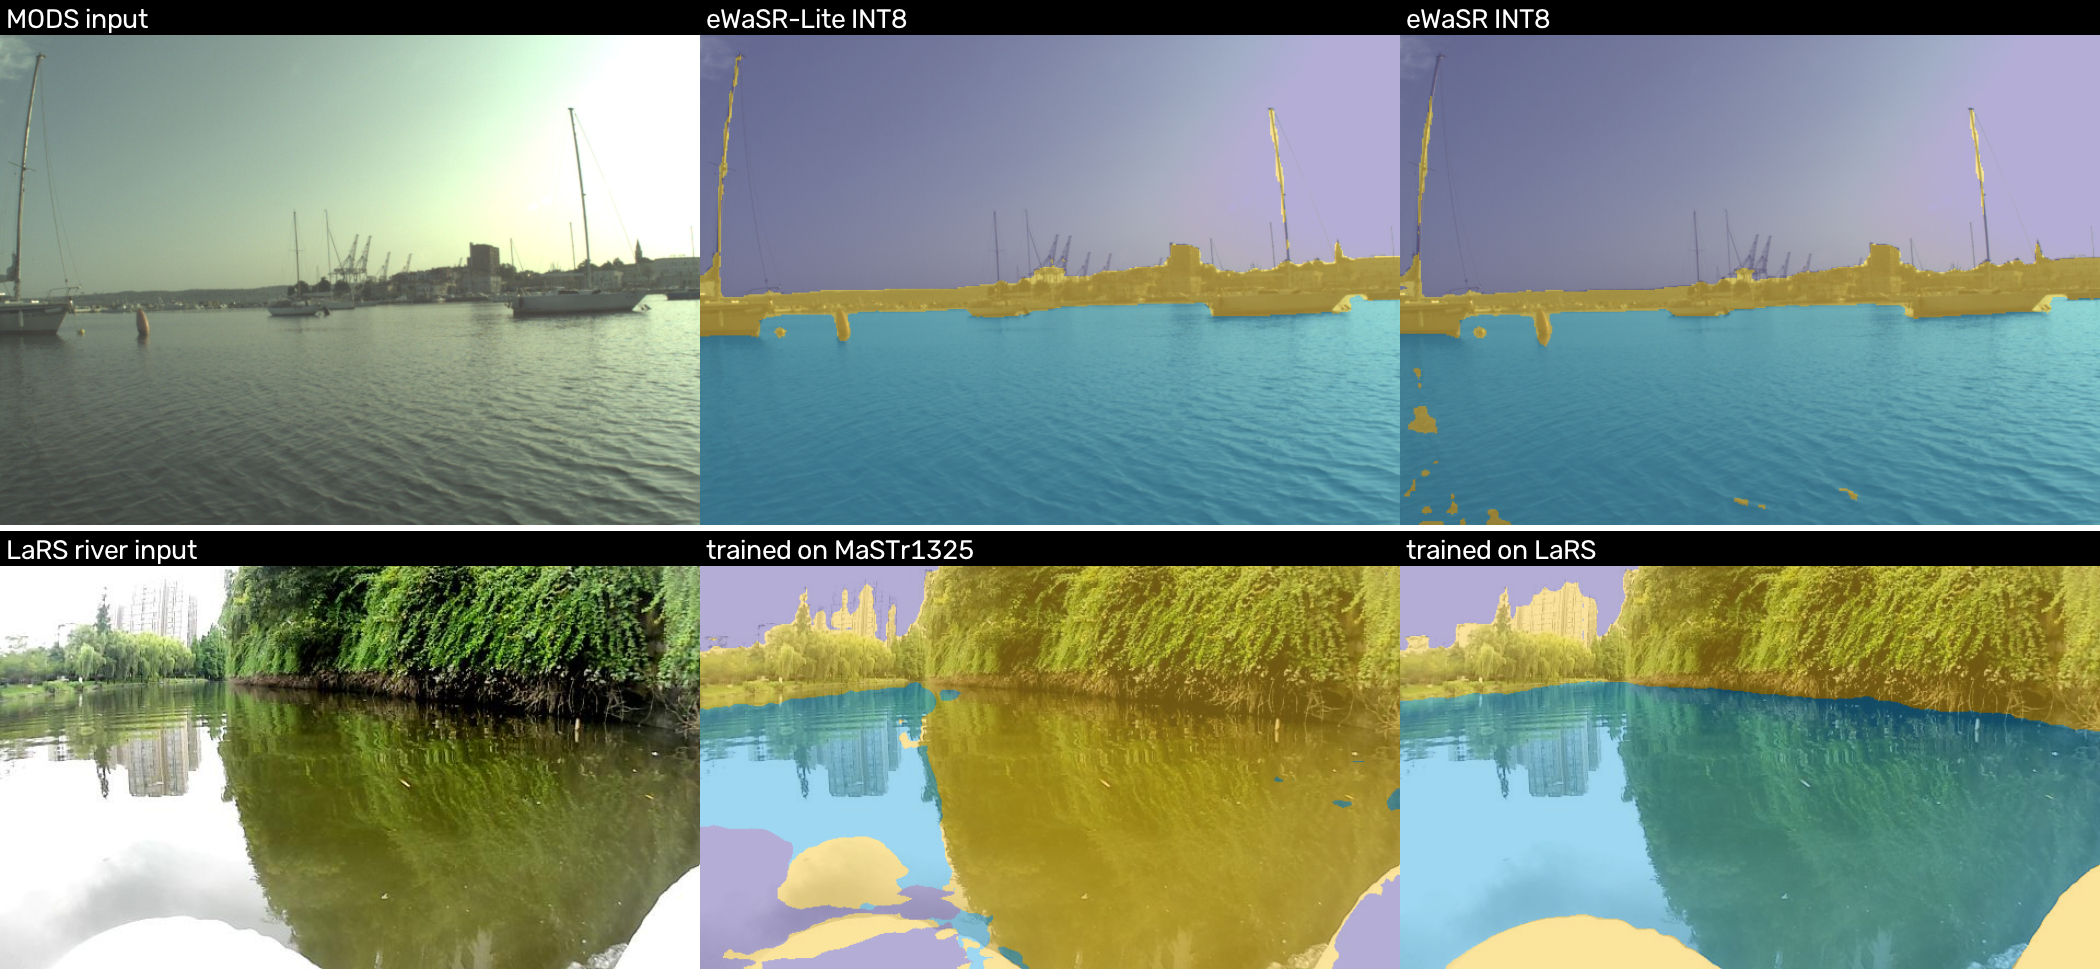
\includegraphics[width=\linewidth]{figs/qual.png}
\caption{Qualitative results (obstacle yellow, water blue, sky purple). Top: MODS frame, INT8 on the Hailo-8L with the same calibration set; eWaSR reports false obstacles on the water in front of the vessel, eWaSR-Lite does not (danger-zone false positives in this frame: 15 vs 0). Bottom: LaRS river frame, eWaSR-Lite in FP32 trained on MaSTr1325 and on LaRS; reflections of the bank are labelled as obstacle by the former.}
\label{fig:qual}
\end{figure}

%==============================================================================
\section{Discussion and Limitations}
\label{sec:disc}
%==============================================================================
\textbf{Why not use the published weights directly?} They are as fast as eWaSR-Lite on the Hailo-8L and more accurate in the danger zone, and they are the model we deploy on our vessel today. Their speed, however, relies on a property of one training run, the vanished MLPs, that our retraining does not reproduce. Any adaptation to a new domain, such as the river scenes of Sec.~\ref{sec:lars}, requires retraining, and with it eWaSR may again need twice the contexts and become sensitive to the calibration set. eWaSR-Lite has the same accuracy, makes the compact graph explicit, and loads the published weights without change.

\textbf{Training recipe.} Our models are 5 points below the published weights in danger-zone F1. We attribute this to the recipe (batch 4 and 100 epochs with mixed precision, versus batch 16 and up to 200 epochs with early stopping), because it affects all variants equally. We also hypothesise that the same recipe difference silences the MLPs: the layer scales share a learning-rate group ($\times20$) with weight decay, and once their task gradient falls below the RMSprop $\varepsilon$, weight decay alone would shrink them exponentially. Testing this, by retraining with the original recipe while logging the layer scales and the optimiser state, is ongoing.

\textbf{Limitations.} (i) Architecture differences should be read against the run-to-run spread; E2 and E6 were trained once. (ii) Our quantization protocol was selected with pixel agreement, which Sec.~\ref{sec:quant} shows to be insufficient; we report task metrics over three calibration sets for the two main models only. (iii) MODS consists of coastal sea scenes; our river results are on LaRS validation with an internal protocol, not the official LaRS benchmark. (iv) We use no IMU; the water edge is 19--21 pixels versus 18 pixels reported with IMU~\cite{tersek2023ewasr}. (v) All on-device tests replay recorded sequences, without closed-loop navigation, and we did not measure power. (vi) Results are for one toolchain version (DFC 3.34); context counts may change with other compilers.

%==============================================================================
\section{Conclusion}
%==============================================================================
On the Hailo-8L of a Raspberry~Pi~5, the speed of eWaSR is set by the number of compiler contexts, which depends on whether the feature-mixer MLPs vanished during training. eWaSR-Lite removes these MLPs: it has 61\% fewer parameters, needs half the contexts, runs 59--70\% faster on the accelerator and 43--55\% faster end-to-end than eWaSR trained with the same recipe (29.7 and 22.7~FPS) with the same MODS accuracy, and its INT8 accuracy does not depend on the calibration set, whereas that of eWaSR can collapse in the danger zone. For low-cost USVs we recommend eWaSR-Lite, or the published eWaSR weights where no retraining is needed, and checking INT8 builds with task metrics on several calibration sets rather than with pixel agreement. Future work includes the original training recipe, IMU-assisted horizon priors, and evaluation on Vietnamese rivers.

\section*{Acknowledgment}
\tbd{}

\bibliographystyle{IEEEtran}
\bibliography{refs}

\end{document}
